% This file was created with tikzplotlib v0.9.12.
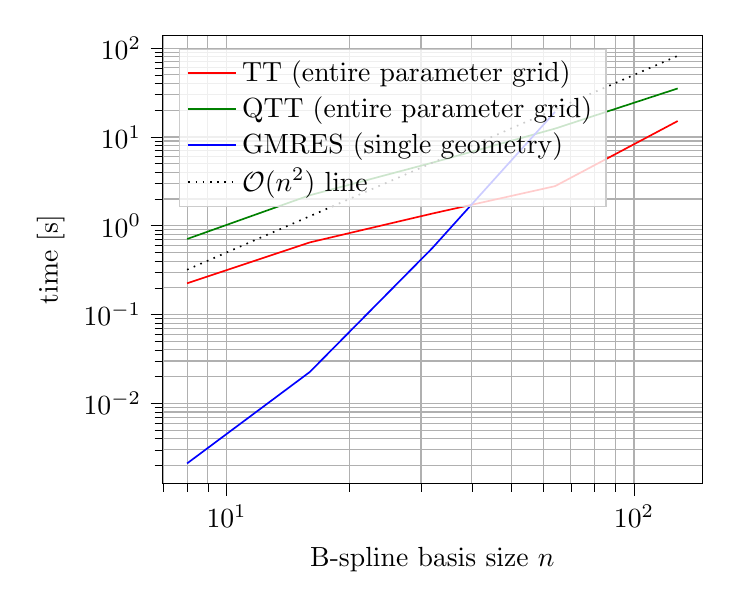
\begin{tikzpicture}

\begin{axis}[
legend cell align={left},
legend style={
  fill opacity=0.8,
  draw opacity=1,
  text opacity=1,
  at={(0.03,0.97)},
  anchor=north west,
  draw=white!80!black
},
log basis x={10},
log basis y={10},
tick align=outside,
tick pos=left,
unbounded coords=jump,
x grid style={white!69.0196078431373!black},
xlabel={B-spline basis size \(\displaystyle n\)},
xmajorgrids,
xmin=6.96440450636899, xmax=147.03338943962,
xminorgrids,
xmode=log,
xtick style={color=black},
y grid style={white!69.0196078431373!black},
ylabel={time [s]},
ymajorgrids,
ymin=0.00124216207423343, ymax=138.95565126356,
yminorgrids,
ymode=log,
ytick style={color=black}
]
\addplot [semithick, red]
table {%
8 0.224968
16 0.649198
32 1.372646
64 2.791932
128 15.105723
};
\addlegendentry{TT (entire parameter grid)}
\addplot [semithick, green!50!black]
table {%
8 0.709622
16 2.205127
32 5.131482
64 12.417141
128 35.166497
};
\addlegendentry{QTT (entire parameter grid)}
\addplot [semithick, blue]
table {%
8 0.002107
16 0.022524
32 0.561367
64 19.150183
128 nan
};
\addlegendentry{GMRES (single geometry)}
\addplot [semithick, black, dotted]
table {%
8 0.32
16 1.28
32 5.12
64 20.48
128 81.92
};
\addlegendentry{$\mathcal{O}(n^{2})$ line}
\end{axis}

\end{tikzpicture}
